\documentclass[preprint,showpacs,preprintnumbers,amsmath,amssymb,pra,aps,superscriptaddress]{revtex4-1}

\usepackage{graphicx}
\usepackage{amsmath}
\usepackage{siunitx}
\usepackage{hyperref}

\begin{document}

\title{Direct Entropy Measurement in a Mesoscopic Quantum System}
\author{Nikolaus Hartman}
\email{nik.hartman@gmail.com}
\thanks{The raw data and Python code used for the figures and analysis can be found at \url{https://github.com/nikhartman/spin_entropy}}
\affiliation{University of British Columbia, Vanouver, BC, Canada}
\author{Saeed Fallahi}
\affiliation{Purdue University, Lafayette, IN, USA}
\author{Geoffrey C. Gardner}
\affiliation{Purdue University, Lafayette, IN, USA}
\author{Christian Olsen}
\affiliation{University of British Columbia, Vanouver, BC, Canada}
\author{Silvia Folk}
\affiliation{University of British Columbia, Vanouver, BC, Canada}
\author{Mohammad Samani}
\altaffiliation{The Hospital for Sick Children, Toronto, ON, Canada}
\altaffiliation{Fields Institute for Research in Mathematical Sciences, Toronto, ON, Canada}
\affiliation{University of British Columbia, Vanouver, BC, Canada}
\author{Michael Manfra}
\affiliation{Purdue University, Lafayette, IN, USA}
\author{Joshua Folk}
\affiliation{University of British Columbia, Vanouver, BC, Canada}
\date{\today}

\begin{abstract}

Measuring the entropy of an electronic state is a powerful tool for identifying its underlying microscopic character.  Such measurements are typically based on bulk properties, such as heat capacity, that are straightforward to observe in macroscopic samples but exceedingly difficult to access in mesoscopic systems that may consist of just a few electrons. Taking advantage of a well-known Maxwell relation, we realize a protocol for entropy-to-charge conversation in a gate-defined GaAs quantum dot that enables an entropy measurement of the first three quantum states in to the dot. The entropy of a single spin ($k_B \ln{2}$) is measured within 8\% accuracy, as is the entropy arising at the magnetic field-driven singlet-triplet crossing for two electrons.

\end{abstract}

\maketitle

%%%%%%% intro material %%%%%%%%%
The thermodynamic properties of electronic systems can offer important insights into the nature of their ground states, and probe exotic quasiparticles that may emerge due to interactions or non-trivial topology.  Systems that are difficult to clearly identify through standard conductance measurements may be studied more in depth if a thermodynamic measurement can be made. For example, the purported non-Abelian exchange statistics of Moore-Read quasiparticles in the $\nu = \frac{5}{2}$ fractional quantum Hall state, or of Majorana quasiparticles in a topological superconductor, are exceedingly difficult to identify from conductance signatures. However, an entropy measurement could clearly distinguish Abelian from non-Abelian quasiparticles \cite{Cooper2009, Smirnov2015}.  Similarly, the two-channel Kondo state that is believed to arise in carefully tuned GaAs devices has so far been identified through a particular temperature dependence in the device conductance \cite{Potok2007}. A more direct test for the two-channel Kondo state would be a confirmation of its entropy ($\frac{1}{2} k_B \ln{2}$), that should remain down to arbitrarily low temperatures \cite{Alkurtass2016}.

%%% figure 1 %%%
\begin{figure}[!]
        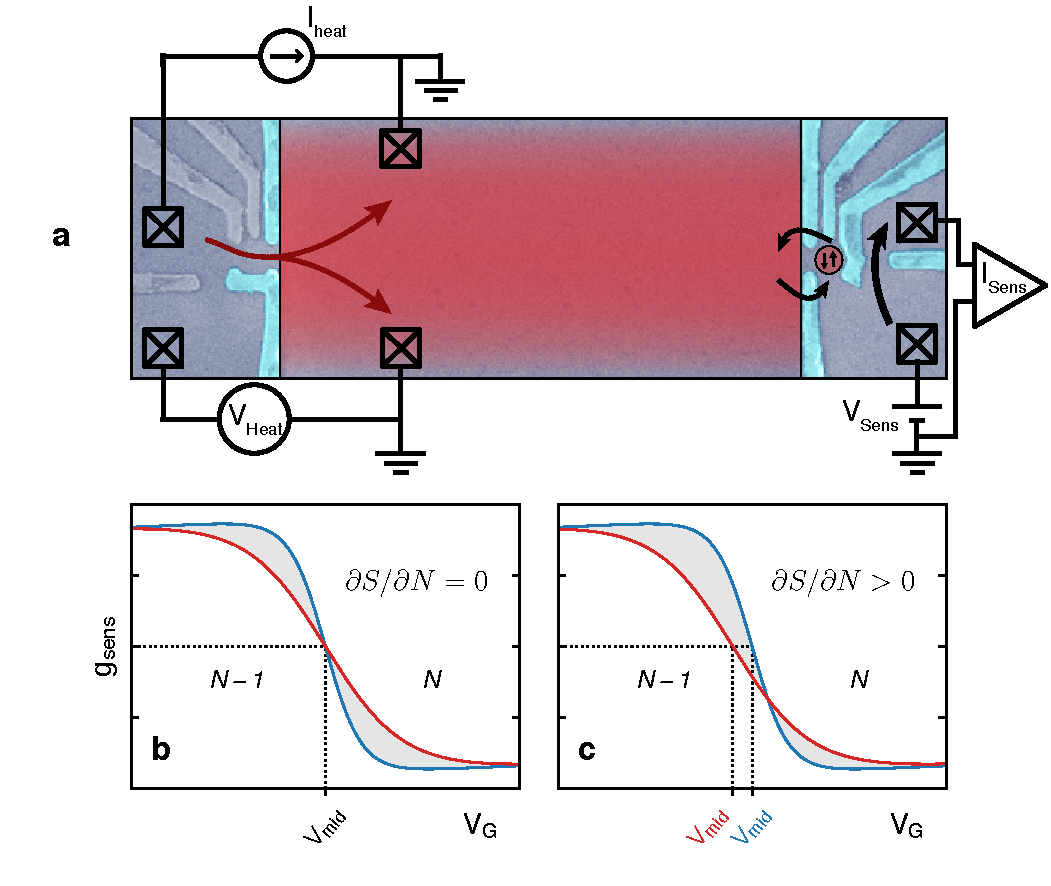
\includegraphics[width=1.0\columnwidth]{../figures/figure_1_no-annotation.pdf}
        \caption{\label{fig:fig1}(a) Scanning electron micrograph of a device similar to the one measured, showing electrostatic gates (blue) used to define a circuit in the 2D electron gas. Grey gates are unused (grounded). Squares show the locations of ohmic contacts to the 2DEG. An electron reservoir is formed between the parallel gates running vertically down the image with a 200nm diameter quantum dot coupled to the right side. The channel can be heated by driving current through the quantum point contact on the left. Electrons tunneling between the reservoir and dot are measured with a capacitively-coupled charge sensor. (b) Calculated charge sensor signal showing a single transition from $N \rightarrow N+1$ electrons at two temperatures ($T_{Red} > T_{Blue}$). (c) Change in the charge sensor signal with respect to temperature. The asymmetry in peak height arises from the shift in $V_0$ which relates to a change in entropy between the $N$ and $N+1$ electron states. In the case of $dS=0$, $dg$ is anti-symmetric about $V_0$.}
\end{figure}

Entropy can be probed effectively in 3D macroscopic samples via measurements of heat capacity, but the heat capacities of single electrons or quasiparticles are much too small to measure directly; even the 2D sheet of quasiparticles in $\nu = \frac{5}{2}$ fractional quantum Hall samples has a heat capacity that vanishes in comparison to that of the host crystal.  Rather than attempt to resolve such infinitesimal signals, the problem can be avoided by converting a change in entropy to changes in charge--a quantity that is easily detected at the single particle level.  Our approach is analogous to the milestone of spin-to-charge conversion, first demonstrated in GaAs quantum dots in 2004, by which undetectably-small magnetic moments of a single spin were transformed into the presence or absence of an electron charge \cite{Elzerman2004, Ono2004}.

In order to accomplish this entropy to charge conversion, we make use of the Maxwell relation
%
\begin{align}
\label{eqn:max}
        \left(\frac{\partial \mu}{\partial T}\right)_{p,N} &= -\left(\frac{\partial S}{\partial N}\right)_{p,T}
\end{align}
%
that connects changes in entropy, $S$, (as well as particle number, $N$, and temperature, $T$) to changes in the chemical potential, $\mu$, a quantity that is simple to measure and control. The fixed pressure condition of Eq.~\ref{eqn:max} is effectively met by working well below the Fermi temperature, $T_F \sim$\SI{5}{\kelvin}, where the pressure is simply the degeneracy pressure \cite{Landau1969}. Refs.~\onlinecite{Cooper2009} and ~\onlinecite{Ben-Shach2013} propose schemes to measure the entropy derivative, $\frac{\partial S}{\partial N}$, of the $\nu = \frac{5}{2}$ state via this Maxwell relation, detecting changes in the quasiparticle chemical potential with temperature.  Our work builds on these ideas to measure the entropy of the few-electron ground states of a quantum dot. Unlike the $\nu = \frac{5}{2}$ quasiparticles described in the theoretical work, the few-electron quantum dot states studied here have an entropy that is well-understood from the spin degree of freedom \cite{Tarucha1996, Ciorga2000, Duncan2000, Lindemann2002, Potok2003, Hofmann2016}. Our experiment demonstrates a direct entropy measurement on a few-particle system; in the future, the method can be easily extended as a probe into the nature of more exotic systems, such as topologically non-trivial Majorana and other non-Abelian states.

The mesoscopic circuit shown in Fig.~\ref{fig:fig1}a realizes an electron reservoir (central region) in thermal equilibrium with a few-electron quantum dot coupled to its right side, whose occupation is measured using an adjacent charge sensing quantum point contact\cite{Staring2007, Frolov2009, Thierschmann2015}. The number of electrons on the dot can be tuned using the gate voltage, $V_G$, to control the chemical potential.  An electron is added to an $N$ electron dot when the chemical potential to add an electron, $\mu_{N+1}$, drops below the Fermi level of the reservoir, $E_F$.  Figure 1b illustrates a such a transition, showing the expected step in charge sensor conductance as a function of $V_G$ and thermal broadening by the reservoir temperature, $T_{res}$. The gate voltage corresponding to midpoint of the transition, $V_0$, marks the chemical potential where the probabilities of finding $N$ or $N+1$ electrons on the dot are equal.

Any entropy change from the $N$ to $N+1$ ground states of the dot should shift the midpoint of the transition, $V_0$, by changing the chemical potential on the dot as in Eq.~\ref{eqn:max}.  Detecting the shift in $V_0$ with respect to temperature (${\propto}\frac{\partial \mu}{\partial T}$), amounts to a measurement of the entropy difference $dS$ between the $N$ to $N+1$ ground states ($dN=1$).  In practice, the shift in $V_0$ with temperature is measured by oscillating $T_{res}$ and monitoring any resulting changes in $g_{sens}$ with a lockin amplifier.  If the transition is broadened but not shifted due to heating ($dS=0$), an antisymmetric lineshape is expected from this lockin measurement.  If the transition is not only broadened but also shifted ($dS,d\mu\neq0$), the change in $g_{sens}$ due to heating will asymmetric, as shown in Fig.~\ref{fig:fig1}c, thus offering a clearly distinguishable signature of entropy for this single charge measurement.

An explanation based on detailed balance is helpful in understanding how the shift in $\mu_{N+1}$ (with respect to $E_F$) upon heating relates to entropy.   In general, electrons tunnel back and forth between the dot and reservoir as long as $\mu_{N+1}$ is within thermal broadening of Fermi level, that is, as long as there are available states in both the dot and the reservoir.  The tunnel rates into and out of the dot, $\Gamma_{in}=\Gamma_{N\rightarrow N+1}$ and $\Gamma_{out}=\Gamma_{N+1\rightarrow N}$, depend on degeneracy of the $N$ and $N+1$ ground states.  Consider the filling of the first electron state at zero magnetic field, a state with a single, unpaired spin-$\frac{1}{2}$ and therefore a degeneracy of 2. An electron tunneling into this state has both spin-up and -down states available.  Tunneling out, the electron (whether spin up or down) must tunnel into reservoir states with the same spin, that is, only half of the reservoir states are available. As a result, $\Gamma_{in} = 2\Gamma_{out}$ when $\mu_{N+1}=E_F$. Extending this logic to a general case gives the same results as derived from detailed balance \cite{Gustavsson2009}, 
%
\begin{align}
	\Gamma_{in} &=  g_{N+1} \Gamma f(E_F - \mu_{N+1}) \label{eqn:rates}\\
	\Gamma_{out} &= g_{N} \Gamma [1 - f(E_F - \mu_{N+1})] \nonumber
\end{align}
%
where $\Gamma$ is a coupling constant, $f$ is the Fermi function, and $g_{N/N+1}$ are the degeneracies of the $N$ and $N+1$ electron states.

The midpoint of the transition between the $N$ and $N+1$ electron states, measured by the charge sensor, occurs when the dot is occupied half the time, that is, when $\Gamma_{in} = \Gamma_{out}$. From Eq.~\ref{eqn:rates}, $\Gamma_{in} = \Gamma_{out}$ occurs when $\mu_{N+1} = E_F$ as long as $g_{N}=g_{N+1}$. When $g_{N}\neq g_{N+1}$, the midpoint of the transition shifts away from $\mu_{N+1}=E_F$ by an amount that depends on the broadening of the Fermi function, and therefore on $T$.   Thus, a measurement of how the midpoint of the transition ($V_0$) shifts with T allows the ratio $g_{N+1}/g_{N}$ to be determined, which itself is related to $dS$ through the Boltzmann entropy formula, $S_{N}=k_{B} \ln{g_N}$.  The relationship between degeneracies and tunnel rates was recently explored in a time-resolved measurement \cite{Hofmann2016}.  The thermal technique presented here extends the measurement of entropy (degeneracy) to a wider set of applications, where the tunneling process may not be convenient or even possible to observe directly.

%%% fab/measurement details %%%
The device was built on a AlGaAs/GaAs heterostructure, hosting a 2D electron gas with density and mobility at \SI{300}{\milli\kelvin} (determined on a separate chip) of \SI{2.42e11}{\per\square\centi\metre} and \SI[per-mode=symbol]{2.56e6}{\square\centi\metre\per\volt\per\second}.   Mesas and NiAuGe ohmic contacts to the 2DEG were defined by standard photolithography techniques, then \SI{10}{\nano\metre} of $\mathrm{HfO_2}$ was deposited via atomic layer deposition to improve the gating stability to the device. Electron beam lithography followed by evaporation of \SI{20}{\nano\metre} of Ti/Au defined the fine gate structures, including the \SI{200}{\nano\metre} diameter quantum dots. The measurement was carried out in an dilution refrigerator with a base temperature of \SI{14}{\milli\kelvin}.

%%%%%%%%%%%%%%%%%%%%%%%

%%% figure 2 %%%
\begin{figure}[!]
        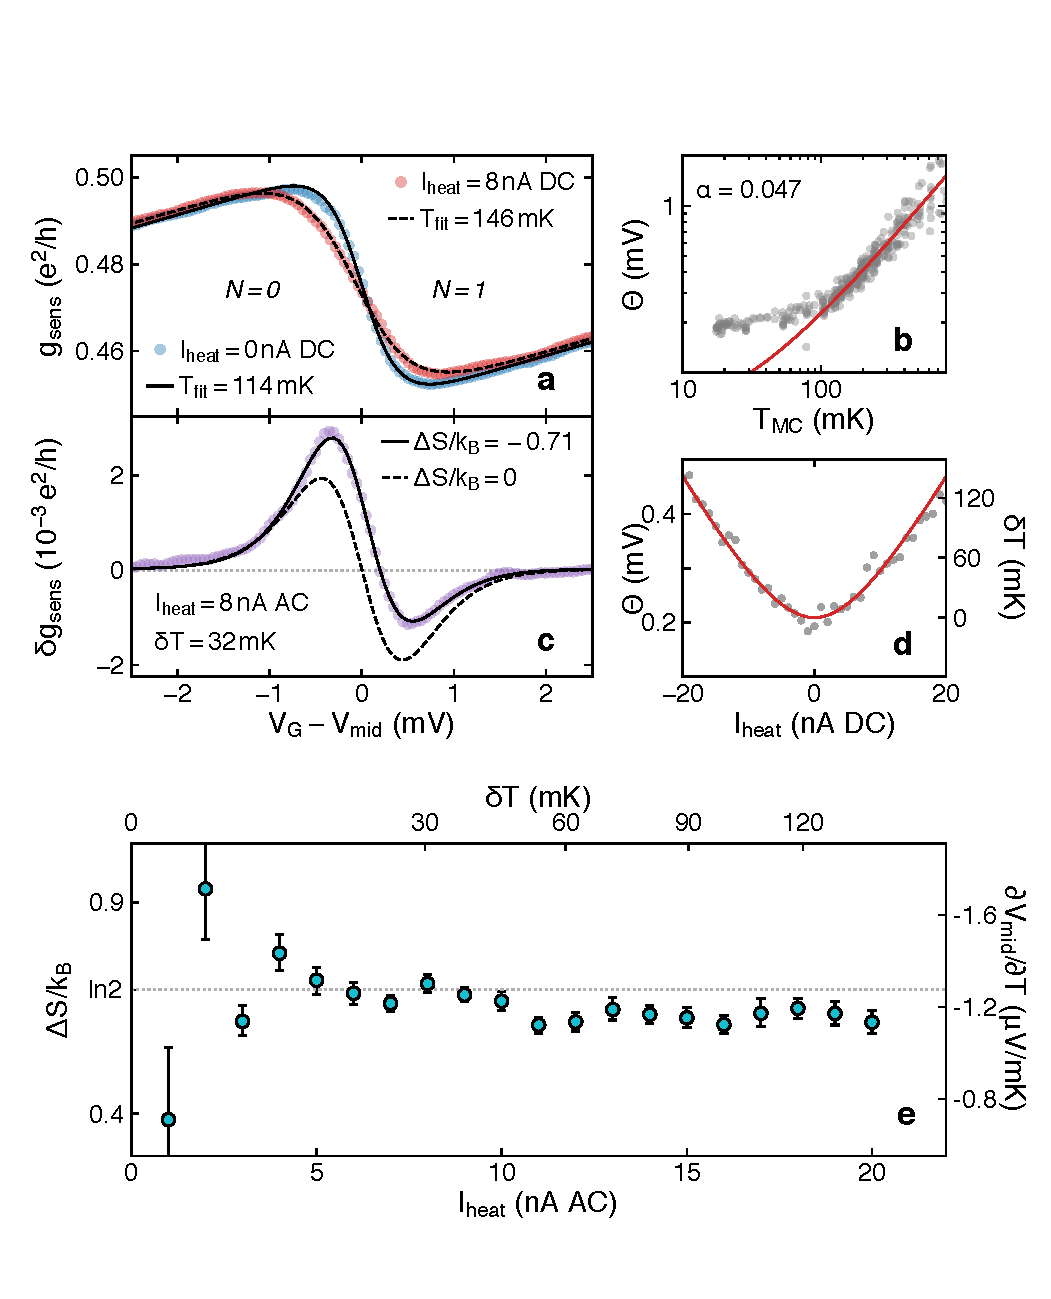
\includegraphics[width=1.0\columnwidth]{../figures/figure_2.pdf}
        \caption{\label{fig:fig2}(a) Charge sensor data for $N=0 \rightarrow 1$ at 100 and 160mK. Temperature is set by DC current through the QPC heater. (b) Lockin measurement of $dg_{sens}$ with $dT \sim 60mK$. Fits to $dg$ are shown with $\delta$ as a free parameter (solid) and $\delta=0$ (dashed) (c) Transition width, $\Theta$, as a function of mixing chamber temperature. The highlighted, linear region is where the tunnel rates are determined only by temperature broadening. The lever arm $\alpha$ is calculated by fitting a straight line to this region. (d) $\Theta$ as a function of DC current through the QPC heater. Linear fit is used to convert between $I_{heat}$ and $dT$, with $R_{QPC} = $ \SI{20}{\kilo\ohm} (e) Change in entropy as a function of AC current through the QPC heater. Top axis shows corresponding $dT$. Right axis shows shift in $V_0$ per unit temperature.}
\end{figure}

%%% device setup %%%
Using the gates on the right side of Fig~\ref{fig:fig1}a, the quantum dot was tuned such that the source was tunnel coupled to the reservoir with the drain closed. The charge sensing QPC was tuned to a conductance of ${\sim}e^2/h$, where conductance was most sensitive to charge on the dot. A small DC voltage bias was applied across the QPC and the measured current was used to calculate the sensor conductance. The reservoir temperature was controlled by varying the mixing chamber temperature or Joule heating through the QPC on the left side of the channel. In the latter case, the QPC was fixed at \SI{20}{\kilo\ohm} and biased with an AC or DC current source. The Joule heating setup gives fast control of the temperature (up to \SI{100}{\hertz}) while keeping the voltage drop across the reservoir negligibly small.

%%% figs 2a and b %%%
Fig.~\ref{fig:fig2}a shows the charge sensor conductance as the first electron is added to the dot by tuning $V_G$, at two different temperatures. The higher temperature transition curve is noticeably broadened by the increased temperature. Assuming the source barrier is sufficiently large, $\Gamma_{in/out}$ are broadened only by the temperature of the reservoir and the conductance takes the form,
%
\begin{align}
\label{eqn:g}
        g_{sens}(V,\Theta) &= G_0 \tanh\left(\frac{V-V_0(\Theta)}{2\Theta}\right)  \\
                        &\quad + G_1\left[V-V_0(\Theta)\right] + G_2 \nonumber
\end{align}
%
where $\Theta = \frac{k_B T}{\alpha e}$, $\alpha$ is the lever arm for the quantum dot plunger gate, and $G_1$ is determined by the cross capacitance between the sensor gates and the plunger gate. The dependence of $V_0$ on $\Theta$ captures any shift in $\mu$ due to a change in entropy (degeneracy) across the transition. Fits to Eq.~\ref{eqn:g} are seen, in addition to the sensor data, in Fig.~\ref{fig:fig2}a. From these fits the transition width, $\Theta$, can be extracted. In Fig.~\ref{fig:fig2}b $\Theta$ is plotted as a function of mixing chamber temperature, $T_{MC}$. From this plot, it is clear that Eq.~\ref{eqn:g} holds when $T_{MC}\gtrsim$ \SI{100}{\milli\kelvin}. For this reason, the mixing chamber temperature remains fixed at \SI{100}{\milli\kelvin} for the remainder of this work. Fitting high temperature data in Fig.~\ref{fig:fig2} to the definition of $\Theta$ (with $T=T_{MC}$) yields $\alpha$, making it possible to convert from $V_G$ to $\mu$.

%%% figs 2c and d%%%
Data in Fig.~\ref{fig:fig2}c, and the corresponding fits, show how $dS$ was measured across a single charge transition. Fluctuations in $g_{sens}$, were measured as $T_{res}$ was varied using Joule heating with an AC current source ($f_{Heat} =$ \SI{48.7}{\hertz}). The change in $T_{res}$ is given by $dT \sim I^{AC}_{Heat} \sim \sin^2(2\omega t)$. A calibration for $dT$, using $\alpha$ as measured in Fig.~\ref{fig:fig2}b, can be seen in Fig.~\ref{fig:fig2}c. To avoid thermally accessing excited states of the dot it must be true that $k_B dT \ll \Delta$ where $\Delta$ is the level spacing between the ground and first excited states; which holds for all transitions investigated. 

To acquire $dg_{sens}$, current fluctuations through the charge sensor were measured at $2f_{Heat}$ using a lockin amplifier. Taking a derivative of Eq. \ref{eqn:g} with respect to temperature gives the form of $dg_{sens}$ near a charge transition,
%
\begin{align}
\label{eqn:dg}
        dg_{sens}(V, \Theta) &\propto \left[ \frac{V-V_0(\Theta)}{2\Theta} + \delta \right]\times \\
        				      &\quad\cosh^{-2}\left(\frac{V-V_0(\Theta)}{2\Theta}\right) \nonumber
\end{align}
%
where $\delta=\frac{\partial V_0}{\partial \Theta}$. Using the lever arm to convert $V_0$ to a chemical potential $\mu$, the parameter $\delta$ can be related to the change in entropy through Eq.~\ref{eqn:max},
%
\begin{align}
\label{eqn:delta}
        \delta &= \frac{\partial V_0}{\partial \Theta} = 
        \frac{1}{k_B} \frac{\partial \mu}{\partial T} = 
        -\frac{1}{k_B} \partial S
\end{align}
%
Fits to Eq.~\ref{eqn:dg} are shown for $\delta=0$ and a best fit to $\delta$. From these fits it is clear $\delta\neq0$ is necessary to properly fit the asymmetry in peak height, with the best fit being $\delta \approx \ln{2}$. For an N-electron macrostate on the quantum dot, entropy is given by the Boltzmann entropy,
%
\begin{align}
\label{eqn:S}
        S &= k_B \ln{\Omega}
\end{align}
%
where $\Omega$ is the spin degeneracy of the ground state, equal to the number of microstates available. For the 0-1 transition, $dS =  k_B\ln{2} - k_B \ln{1} = k_B\ln{2}$.

%%% fig 2e %%%
Note that $\delta$ is a fit parameter independent of $dT$ and $\alpha$. Fig.~\ref{fig:fig2}e shows that $dS$, as determined from fits to $dg_{sens}$ data, remains constant over a range of $dT$ ($I^{AC}_{Heat}$). The vertical scale on the right side of Fig. \ref{fig:fig2}e, $\delta$ in units of gate voltage per unit temperature, illustrates the necessity of the lockin measurement; device stability and small signals made it difficult for $delta$ to be determined directly from $g_{sens}$ at different $T$. Without any additional calibration, it is possible to measure $dS$ directly from the lockin amplifier signal, $dg_{sens}$.

%%% figure 3 %%%
\begin{figure}
        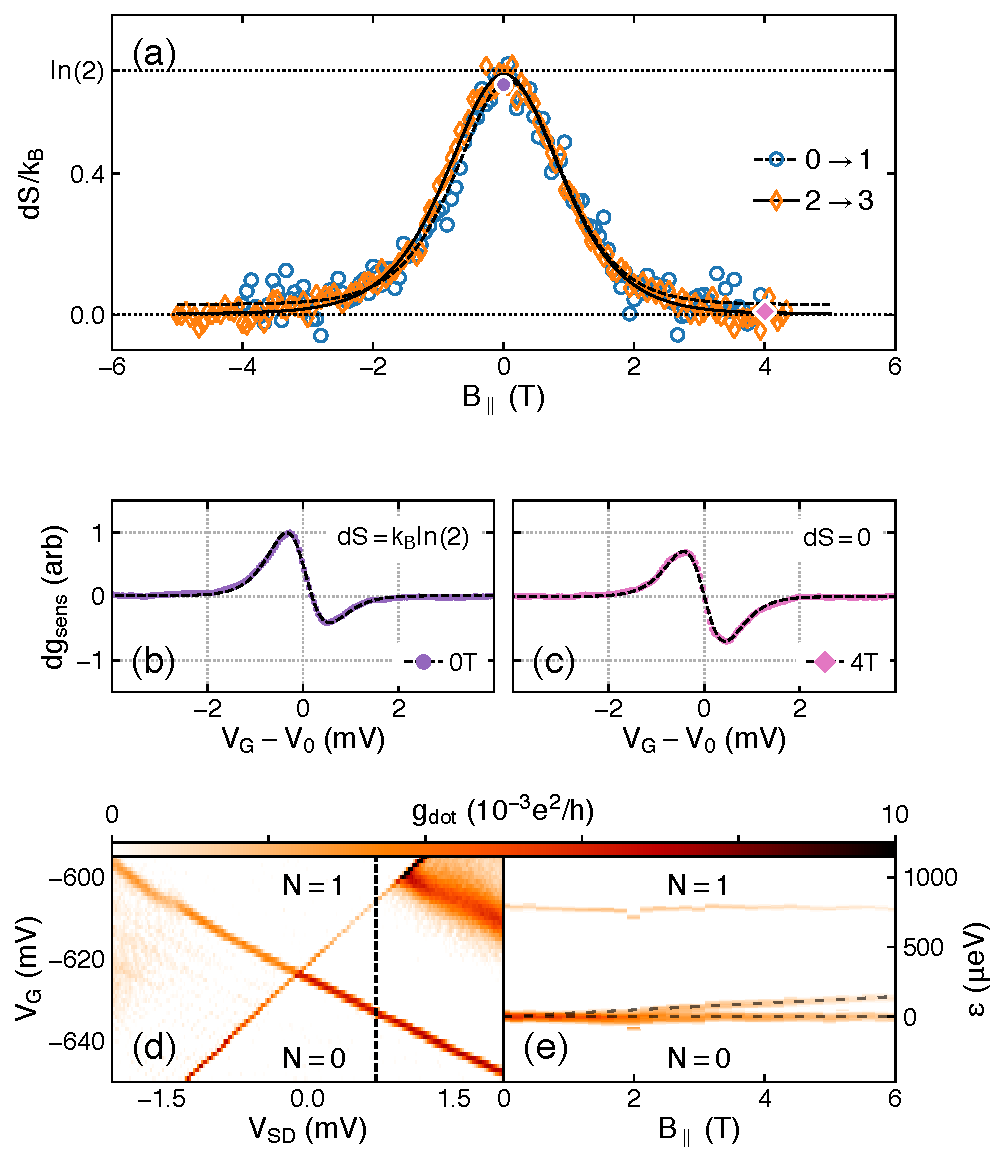
\includegraphics[width=1.0\columnwidth]{../figures/figure_3.pdf}
        \caption{\label{fig:fig3}(a) Transport data through the quantum dot showing the $N=0 \rightarrow 1$ transition. The first excited state, near $V_{SD} = $ \SI{1}{\milli\electronvolt}, is well-above all other energy scales in the measurement. Dashed line at $V_{SD}$ = \SI{700}{\micro\electronvolt} shows where data in (b) are taken. (b) Fixed bias transport data showing fits to the Zeeman splitting of the ground state energy from which $g = -0.44$ is extracted. (c) Change in entropy, determined from $dg$ fits at varying parallel magnetic field. The $N=0 \rightarrow 1$ and $2 \rightarrow 3$ data are overlaid here to show the similar behavior of these states at low field. (d) and (e) show characteristic $dg$ traces from which the data in (c) were extracted. These data points are show as large markers in (c)}
\end{figure}

To confirm that the measured signal derives from the electron spin, the behavior of $dS$ was investigated as a function of parallel magnetic field. Fig.~\ref{fig:fig3}c shows $dS$ as a function of applied field for the 0-1 and 2-3 electron transitions. The 2-electron ground state is a spin singlet, while the 3-electron ground state is same singlet with an additional unpaired electron, making the field-dependent behavior of these transitions identical where $g \mu_{B} B$ is less than the excited state energies. Zeeman splitting, measured directly in Fig. \ref{fig:fig2}b, lifts the spin degeneracy of the unpaired electrons and the entropy of the 1- and 3- electron ground states goes to zero with increasing field

The behavior of $dS$ as a function of magnetic field can be understood using the Gibbs entropy,
%
\begin{align}
\label{eqn:gibbs}
        S &= k_B \sum_{i=\pm} p_{i}(B, T) \ln{ p_{i}(B,T) }
\end{align}
%
where $p_{i}(B, T)$ is the probability of the system being in the i$^{th}$ spin state at a given field and temperature.  For states with a single unpaired electron, $p_{i}(B, T)$ can be written as a two-level system,
%
\begin{align}
\label{eqn:p}
        p_{\pm}(B, T) &= \frac{1}{1+ e^{\mp \frac{g\mu_B B}{k_B T}}}
\end{align}
%
where $\pm$ represent the spin up/down states. Fits to Eqs.~\ref{eqn:gibbs} and \ref{eqn:p} are shown in Fig \ref{fig:fig3}c for each transition. The fits allow for peak height, g-factor, and a vertical offset as free parameters with $T$ fixed at $T_{MC}$. From these fits we find $dS(B=0)=0.92 \ln{2}$ and $g=-0.33$ for the 0-1 transition.  Discrepancy between $g$ and the result shown in Fig. \ref{fig:fig3}b, is understood from the change in shape of the quantum dot when tuning between the $g_{dot}$ and $g_{sens}$ measurements [cite?]. The entropy agrees well with the expected $k_{B} \ln{2}$ at zero-field and goes to zero as expected with $B_{\parallel}$

%%% figure 4 %%%
\begin{figure}
        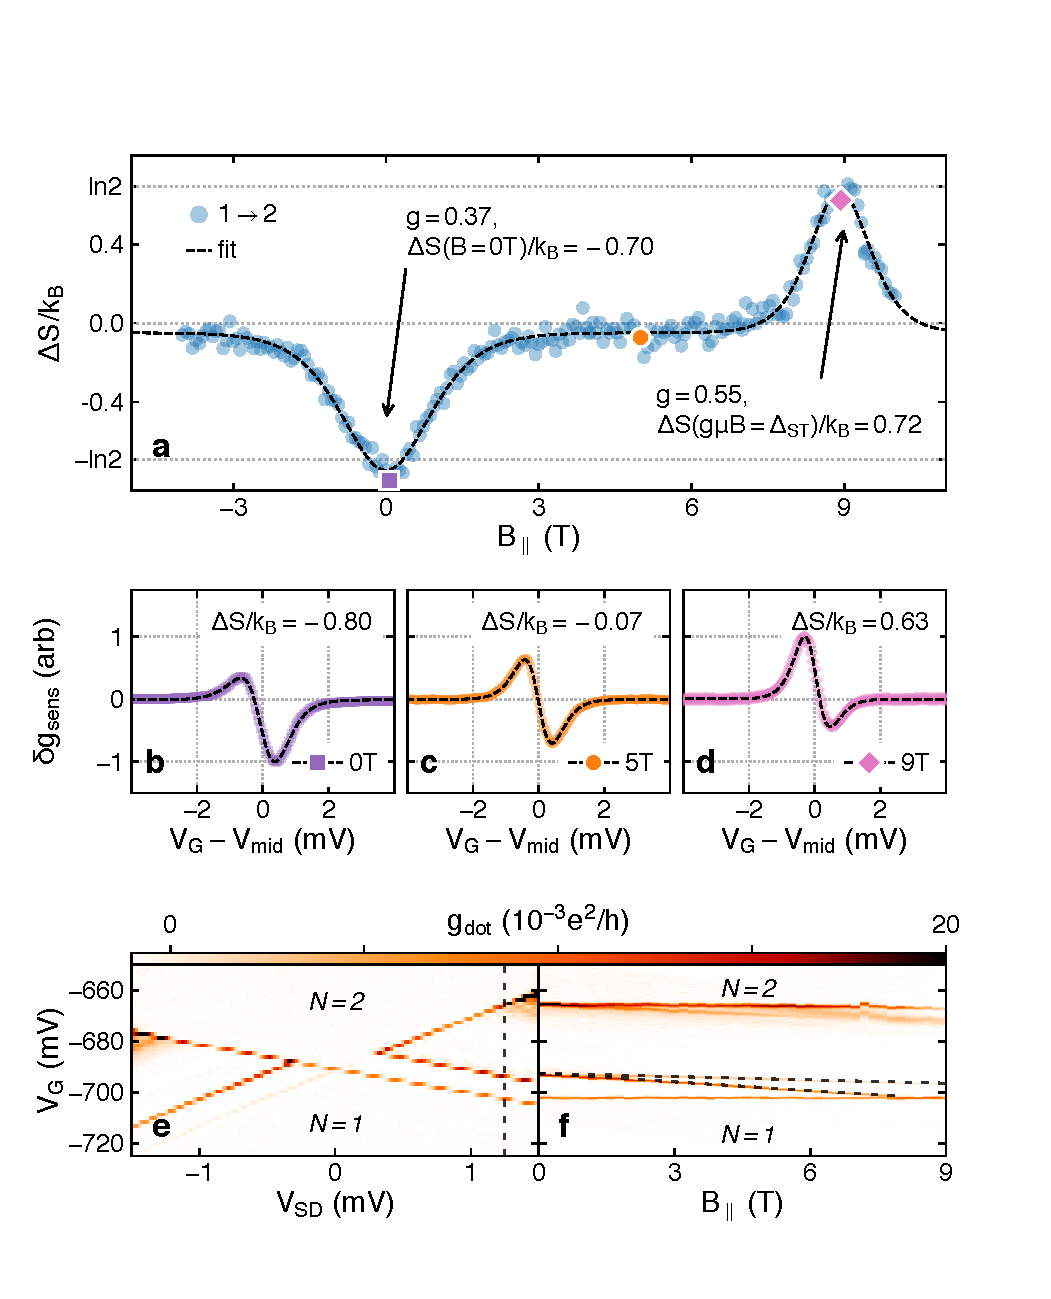
\includegraphics[width=1.0\columnwidth]{../figures/figure_4.pdf}
        \caption{\label{fig:fig4}(a) (a) Transport data through the quantum dot showing the $N=1 \rightarrow 2$ transition. Singlet-triplet splitting is roughly \SI{300}{\micro\electronvolt} and depends on applied field. Dashed line at $V_{SD}$ = \SI{1250}{\micro\electronvolt} shows where data in (b) are taken. (b) Fixed bias transport data in parallel field. The triplet level is split into $T_+$, $T_0$, and $T_{-}$ (not visible). At \SI[input-protect-tokens]{\sim 9}{\tesla} $T_+$ becomes degenerate with $S$. $g$ is determined using $T_0$ and $T_+$ fits. (c) Change in entropy, extracted from $dg$ fits at varying parallel field. As the field goes from 0 to 10T, entropy of the 2-electron state goes from $0  \rightarrow \ln{2}$, while the entropy of the 1-electron state goes from $\ln{2} \rightarrow 0$. Fit to this behavior (dashed) is described in the text (d), (e), and (f) show characteristic $dg$ traces from which the data in (c) were extracted. These data points are show as large markers in (c)}
\end{figure}

The low field (\SI{<5}{\tesla}) data in Fig. \ref{fig:fig4}c for the 1-2 electron transition is understood as the inverse of Fig \ref{fig:fig3}c. The 2-electron ground state remains in the spin singlet state with zero entropy while 1-electron ground state entropy goes from $k_B\ln{2}$ to zero due to Zeeman splitting. At high fields, the 1-electron ground state remains non-degenerate, while the 2-electron ground state becomes two-fold degenerate at \SI{9}{\tesla} where the singlet ($S$) and triplet ($T_+$) states cross. The singlet-triplet crossing is seen clearly in Fig.~\ref{fig:fig4}b. 

The entropy for the 1-2 transition can again be fit using Eq.~\ref{eqn:gibbs}, with probabilities given by Eq.~\ref{eqn:p} for the 1-electron states and the following probabilities for the 2-electron singlet-triplet states,
%
\begin{align}
\label{eqn:pst}
        p_{S/T}(B, T) &= \frac{1}{1+ e^{\mp \frac{g\mu_B B - \Delta_{ST}}{k_B T}}}
\end{align}
%
where $\Delta_{ST}$ is the singlet-triplet splitting at zero field. Fitting the data in Fig.~\ref{fig:fig4}c we find $g(B{=}0T)=-0.46$, $g(B{=}9T)=-0.31$, $\Delta_{ST}(B{=}9T)$ = \SI{240}{\micro\electronvolt}, $dS(B{=}0T) = 1.04\ln{2}$, and $dS(B{=}9T) = 1.01\ln{2}$. Each of these values is consistent with data in Figs.~\ref{fig:fig4}a and b as well as previous GaAs dot measurements [cite why g should change in high field]. This fit confirms that the $dS$ signal can be related directly to a tunable degeneracy in the system.

%%% conclusion %%%
The results presented demonstrate a novel technique to measure the entropy of few-particle states in mesoscopic devices. The measurement was used to investigate the well-understood spin degeneracy of the few-electron ground states states in a GaAs quantum dot. The entropy signal is confirmed by tuning the entropy as a function of applied magnetic field. Future work may take advantage of this strategy to look for thermodyanmic signatures of non-trival electron and quasiparticle states, eliminating the uncertainty found in typical transport data.

%\acknowledgments
% Everyone I might acknowledge is currently an author. Consider moving someone here.

\bibliography{qdentropy}{}
\bibliographystyle{apsrev4-1}

\end{document}